\documentclass{esannV2}
\usepackage{graphicx}
\usepackage[utf8]{inputenc}
\usepackage{amssymb,amsmath,array}

\usepackage{hyperref}
\usepackage{listings}
\usepackage{enumitem}
\usepackage{graphicx}
\usepackage{float}
\lstset{
  language=bash,
  basicstyle=\ttfamily
}
%***********************************************************************
% !!!! IMPORTANT NOTICE ON TEXT MARGINS !!!!!
%***********************************************************************
%
% Please avoid using DVI2PDF or PS2PDF converters: some undesired
% shifting/scaling may occur when using these programs
% It is strongly recommended to use the DVIPS converters, and to submit
% PS file. You may submit a PDF file if and only if you use ADOBE ACROBAT
% to convert your PS file to PDF.
%
% Check that you have set the paper size to A4 (and NOT to letter) in your
% dvi2ps converter, in Adobe Acrobat if you use it, and in any printer driver
% that you could use.  You also have to disable the 'scale to fit paper' option
% of your printer driver.
%
% In any case, please check carefully that the final size of the top and
% bottom margins is 5.2 cm and of the left and right margins is 4.4 cm.
% It is your responsibility to verify this important requirement.  If these margin requirements and not fulfilled at the end of your file generation process, please use the following commands to correct them.  Otherwise, please do not modify these commands.
%
\voffset 0 cm \hoffset 0 cm \addtolength{\textwidth}{0cm}
\addtolength{\textheight}{0cm}\addtolength{\leftmargin}{0cm}

%***********************************************************************
% !!!! USE OF THE esannV2 LaTeX STYLE FILE !!!!!
%***********************************************************************
%
% Some commands are inserted in the following .tex example file.  Therefore to
% set up your ESANN submission, please use this file and modify it to insert
% your text, rather than staring from a blank .tex file.  In this way, you will
% have the commands inserted in the right place.

\begin{document}
%style file for ESANN manuscripts
\title{Clasificación de alimentos mediante la detección de estímulos aplicando técnicas de aprendizaje automático}

%***********************************************************************
% AUTHORS INFORMATION AREA
%***********************************************************************
\author{
Luis Fernández Freire \and
\qquad Raúl Martín Hernández\and
Alejandro Benimeli Miranda\and
Rodrigo Juez Hernández
%
% Optional short acknowledgment: remove next line if non-needed
%\thanks{This is an optional funding source acknowledgement.}
%
% DO NOT MODIFY THE FOLLOWING '\vspace' ARGUMENT
\vspace{.3cm}}
%***********************************************************************
% END OF AUTHORS INFORMATION AREA
%***********************************************************************

\maketitle

\begin{abstract}
Este estudio investiga un conjunto de sensores de gas que generan datos en forma de series de tiempo en las cuales deberemos evaluar cuando se introduce un estímulo y clasificar dicho estímulo entre las clases plátano, vino y ruido de fondo. Los datos se han tratado y modificado para adaptarlos al problema de clasificación. Para la clasificación se han probado diversos métodos de machine learning tradicionales usando optimización de hiperparámetros. Nuestro análisis ha concluido que el clasificador más robusto es Random Forest con una precisión de 0.9962±0.0005, y es también al que menos afecta reducir el tamaño del dataset.
\end{abstract}
\section{Introducción}
El problema que vamos a afrontar en este documento consiste en clasificar instantes de tiempo entre tres clases: vino, plátano y ruido de fondo. Los datos proporcionados consisten en series de tiempo de 8 sensores de tipo MOX, además de la temperatura y humedad. Los sensores están colocados dentro de una habitación y miden cuando se introduce uno de los dos objetos mencionados, o cuando no hay nada y entonces se considera ruido de fondo. Los objetos se introducen siempre una hora después de comenzar el experimento, pero pueden ser eliminados en cualquier momento.
\newline\newline
El dataset \cite{dataset} esta contenido en dos archivos .dat, uno de datos, que contiene todas las mediciones de todas las instancias de tiempo, y otro de metadatos, en el que se indica a qué clase pertenece cada serie, y durante cuánto tiempo se introdujo el alimento. Ambos datasets se relacionan mediante una id, donde cada serie tiene un conjunto de instantes de tiempo asociados.\\

\section{Análisis exploratorio de los datos}\label{section:analisisDatos}

Antes de empezar a crear atributos y seleccionar los más importantes vamos a analizar los datos que se han extraído en la fase de experimentación. Para empezar, en los datos contamos con las 3 clases mencionadas anteriormente, que son Plátano, Vino o Ruido (Banana, Wine o Background en inglés).
\newline\newline
Para cada clase hay un número diferente de series, que se puede ver en la Figura \ref{fig:proporcionClases}. Para cada una de estas clases hay una proporción diferente de muestras de tiempo, visible en la Figura \ref{fig:proporcionInstanciasClases}. Este desbalance se debe a que en cada serie donde se introduce plátano o vino, hay un tiempo antes y después donde la muestra no está presente, por lo que hemos considerado que dichas instancias de tiempo deben ser de la clase Ruido. Hemos tenido esto en cuenta en la Sección \ref{section:preprocesado}, donde se trata el preprocesado de datos.
\newline\newline
Hemos encontrado que aunque en el fichero metadata figure una serie número 95, no existen instancias de tiempo asociadas a dicha serie en el fichero dataset. Esto se ha tenido en cuenta a la hora de generar la Figura \ref{fig:proporcionClases}.\\

\begin{figure}[ht]
\centering
\begin{minipage}{.48\textwidth}
  \centering
  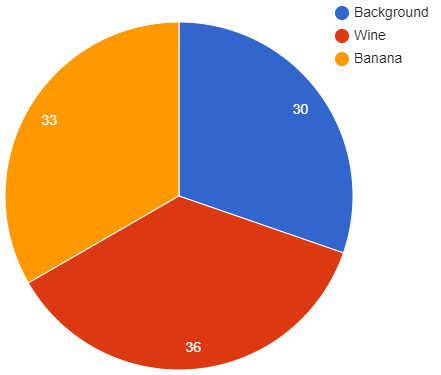
\includegraphics[scale=0.35]{figuras/proporcionClases.png}
  \caption{Número de series de cada clase.}
  \label{fig:proporcionClases}
\end{minipage}%
\quad
\begin{minipage}{.48\textwidth}
  \centering
  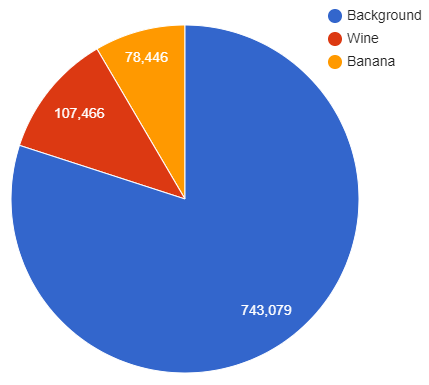
\includegraphics[scale=0.35]{figuras/proporcionInstanciasClases.png}
  \caption{Número de instantes de tiempo de cada clase.} \label{fig:proporcionInstanciasClases}
\end{minipage}
\end{figure}

\noindent
Hemos llevado a cabo un análisis estadístico de los valores recogidos por cada sensor, y hemos conseguido unas gráficas que nos han dado una información muy relevante, presentes en la Figura \ref{fig:mediasSensoresPorSerie}. En estas gráficas podemos ver cómo todos los sensores tienen un comportamiento razonable dentro de un umbral. En cambio el sensor 5 tiene unos extraños picos que seguramente se deban a que es defectuoso, y podrían afectar a la tarea de clasificación.

\begin{figure}[H]
\centering
\begin{minipage}{.5\textwidth}
  \centering
  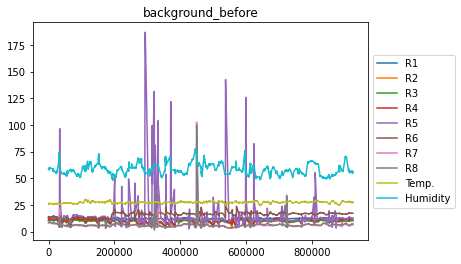
\includegraphics[width=\linewidth]{figuras/mediasSensoresPorSerie_background1.png}
\end{minipage}%
\begin{minipage}{.5\textwidth}
  \centering
  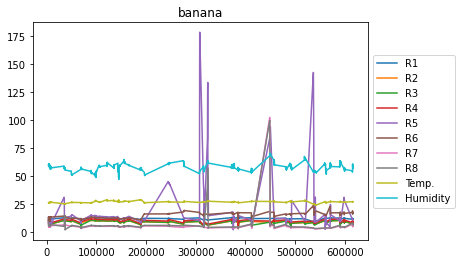
\includegraphics[width=\linewidth]{figuras/mediasSensoresPorSerie_banana.png}
\end{minipage}
\caption{Valores de cada sensor por cada instancia de tiempo.}
\label{fig:mediasSensoresPorSerie}
\end{figure}
\noindent
Gracias a los datos del experimento anterior, hemos calculado estadísticas para cada clase, por cada sensor. En la Figura \ref{fig:mediasSensores} podemos ver las medias y varianzas de cada sensor para cada clase, generada con matplotlib \cite{matplotlib}. Es importante remarcar que se han anotado dos clases más, en las que se consideran diferentes tipos de riudo antes y después de meter los estímulos. Esto es así ya que en algunas observaciones hemos percibido que después de insertar el estímulo algún tipo de residuo afecta a los sensores. Esto se puede observar en la Figura \ref{fig:mediasSensores}, en la que  en ciertos sensores la varianza de background es menor a la de background\_after.\newline
\begin{figure}[H]
    \centering
    \centering
    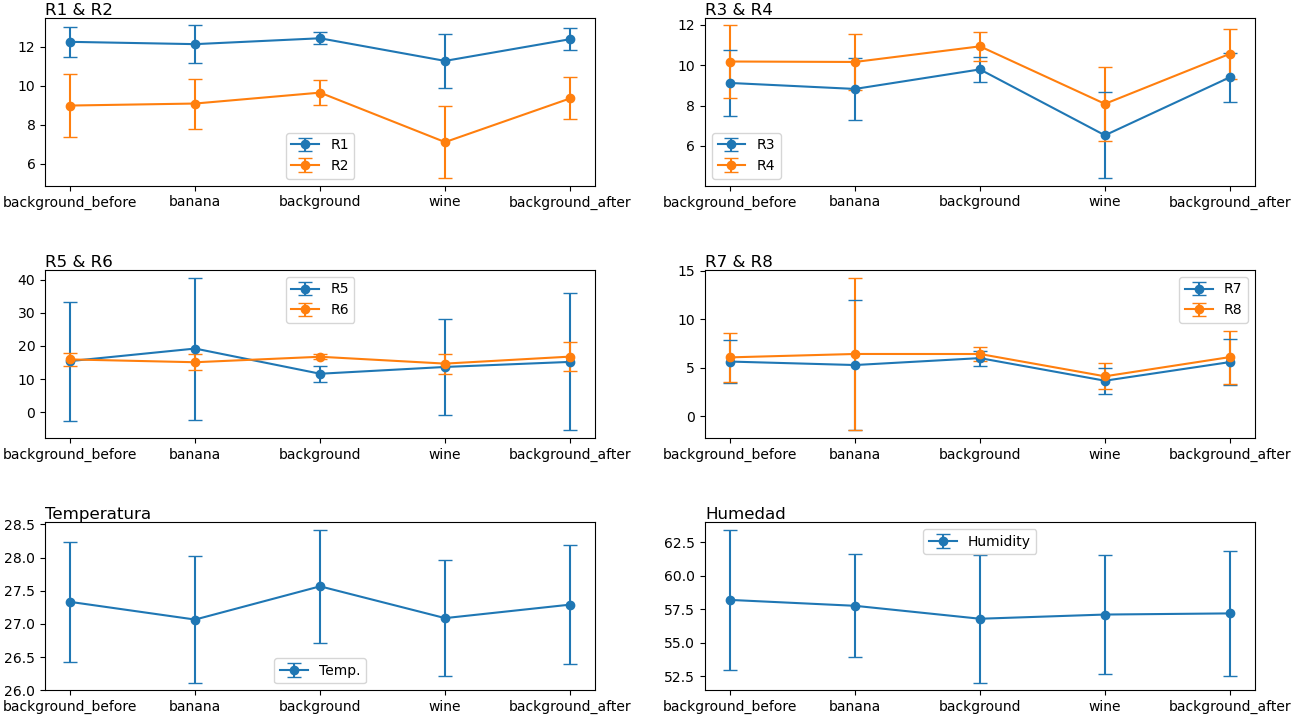
\includegraphics[width=\linewidth]{figuras/mediasSensores.png}
    \caption{Medias y varianzas de cada sensor.}
    \label{fig:mediasSensores}
\end{figure}
\noindent
Por último podemos remarcar que este análisis resulta útil sobre todo para fijarnos en que existe algún tipo de correlación entre algunos sensores de tipo MOX, algo en lo que indagamos con más profundidad en la Sección \ref{section:eliminacionAtributos}.

\section{Preprocesado de datos y propuestas de nuevos atributos}
\label{section:preprocesado}
Antes de añadir o quitar atributos hemos generado el dataset principal en el que cada instante de tiempo tiene asociada una clase, juntando la información presente en ambos datasets. Hemos considerado que las instancias de tiempo antes de introducir la muestra y después de retirarla son background. Esto hace que el dataset quede muy desbalanceado, por lo que se hace un muestreo aleatorio para que las clases tengan el mismo número de filas a la hora de clasificar.
\newline\newline
Una vez hecho esto, hemos adaptado el dataset para poder clasificar instantes de tiempo, aprovechando la técnica de ventanas de tiempo. Estas ventanas constan de al menos 3 muestras de tiempo anteriores a cada instancia a evaluar, y dentro de un margen de tiempo que, después de una rápida experimentación hemos determinado que debe ser de 3 minutos. Las ventanas que no cumplen estas condiciones se establecen como NaN, y posteriormente se eliminan, junto con las columnas de tiempo e id.
Todo el procesado de datos se ha realizado usando las librerías Numpy \cite{numpy} y Pandas \cite{pandas}.

\subsection{Nuevos atributos}\label{section:nuevosAtributos}
Gracias a los resultados observados en la Figura \ref{fig:mediasSensores}, hemos considerado que añadir los siguientes atributos estadísticos facilitarían la tarea de clasificación. Para cada sensor hemos añadido los siguientes atributos:

\begin{figure}[H]
\begin{minipage}{.55\textwidth}
    \begin{itemize}
    \item Media: Este atributo se utiliza para representar el valor medio que ha tenido la ventana durante los últimos minutos.
    \item Desviación Típica: Este valor representa la variación le las mediciones en la ventana de tiempo ya que, como se puede ver en la Figura \ref{fig:timeseries} (generada gracias al código extraído de \cite{visualizacion_series}), cuando se introduce la muestra de vino la varianza de las mediciones se ve incrementada.
    \item Min y Max: Estos valores apoyan a la desviación típica para indicar el umbral que ha alcanzado la ventana.
    \item Pendiente: Este atributo resulta de alta importancia ya que consideramos que las ventanas que se encuentran en los cambios entre background y muestras de alimentos pertenecen a la clase del alimento.
    \end{itemize}
\end{minipage}%
\quad
\begin{minipage}{.4\textwidth}
    \centering
    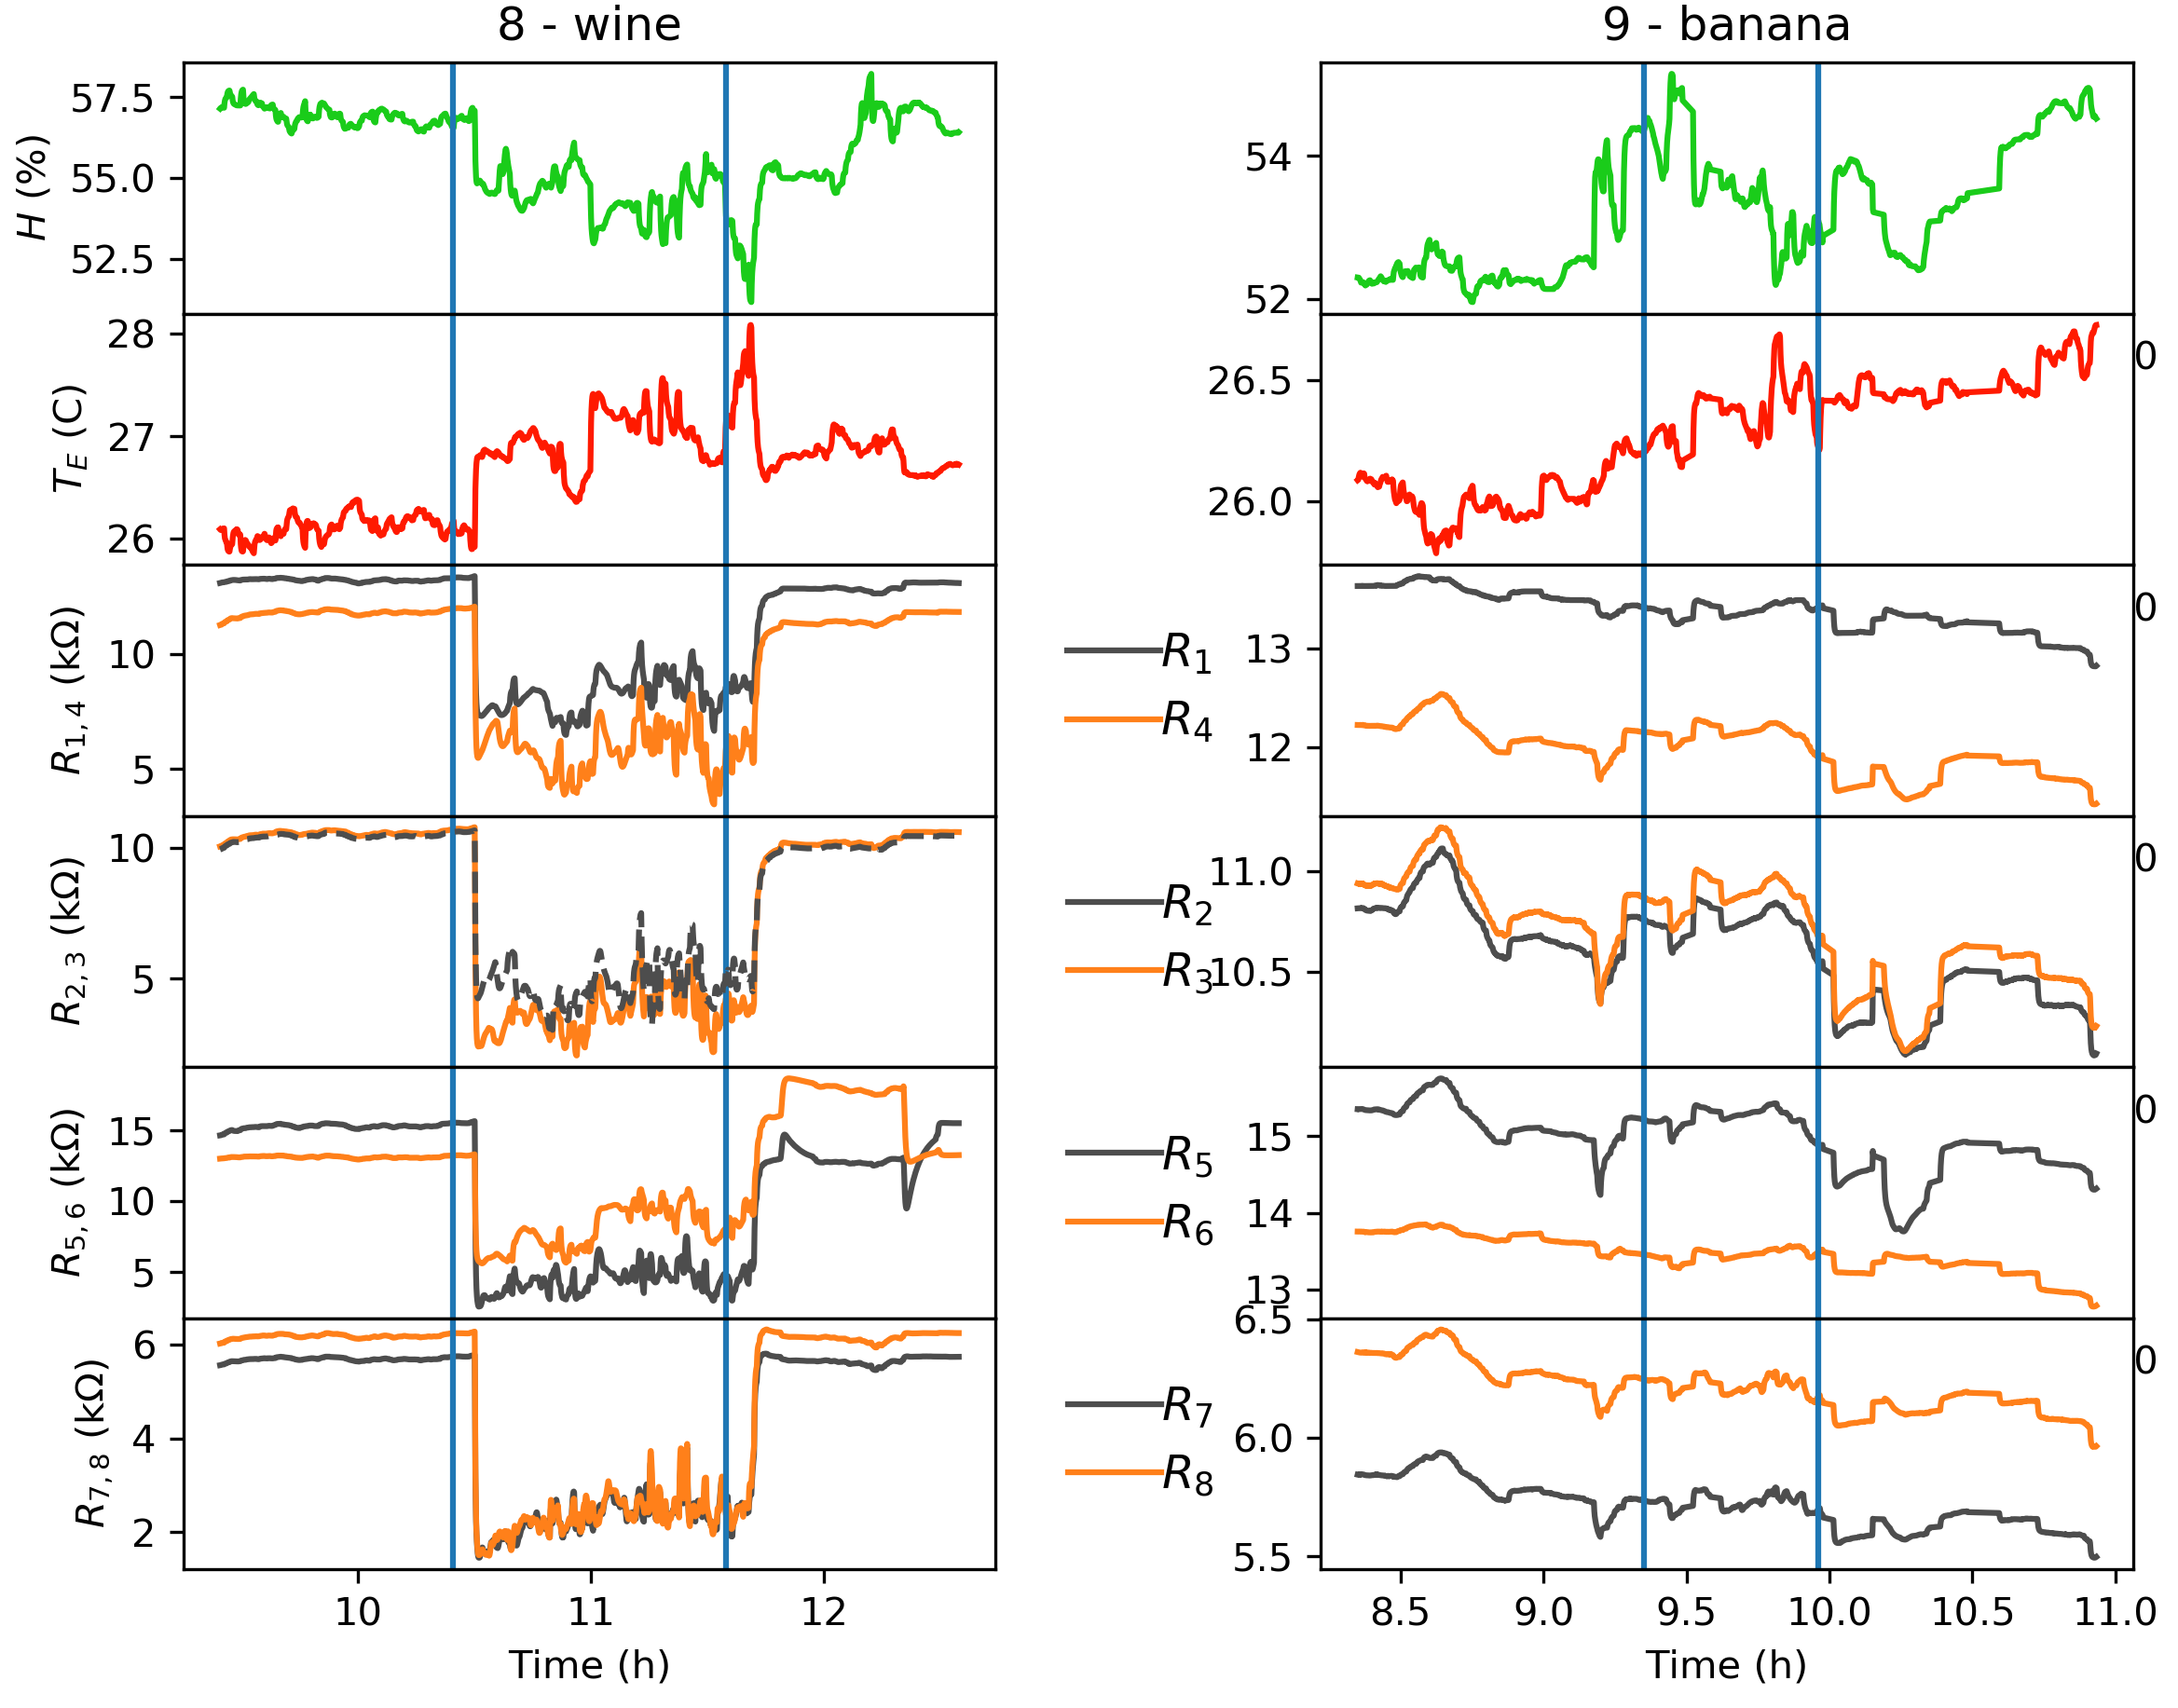
\includegraphics[scale=0.18,trim={1.5cm 0 33.3cm 0},clip]{figuras/justificacion_atributos_propuestos.png}
    \caption{Visualización de la serie 8 por cada sensor.}\label{fig:timeseries}
\end{minipage}%
\end{figure}

\subsection{Eliminación de atributos}\label{section:eliminacionAtributos}
Añadir 5 atributos por cada sensor resulta en unos 60 atributos. Esto puede resultar problemático en lo que a tiempo de ejecución respecta, y por ello hemos reducido la dimensionalidad gracias a las conclusiones extraídas en las secciones anteriores.
\newline\newline
En la Sección \ref{section:analisisDatos} hemos visto que el sensor 5 está defectuoso, por lo que hemos eliminado todos sus atributos (R5, R5mean, R5std...).
\newline
Una vez hecho esto, vamos a probar a visualizar la matriz de correlación de todos los atributos. Esta información está presente en la Figura \ref{fig:corrMal}. Aquí los píxeles con valores muy cercanos a 1 o -1 indican una alta correlación entre atributos, lo que significa que éstos son redundantes entre sí.

\begin{figure}[H]
\centering
\begin{minipage}{.48\textwidth}
  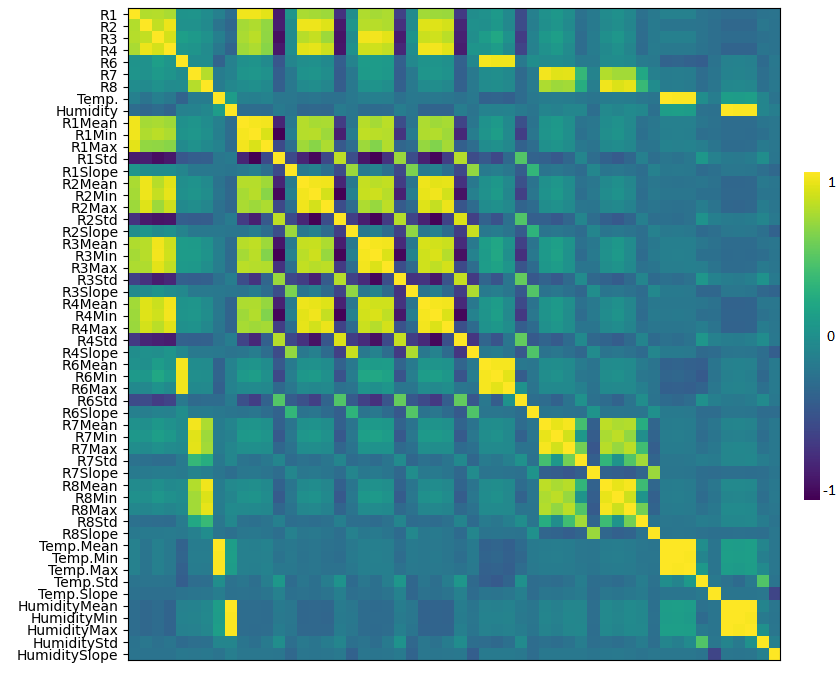
\includegraphics[width=\linewidth]{figuras/Correlation_mal.png}
  \caption{Matriz de correlación antes de borrar atributos.}\label{fig:corrMal}
\end{minipage}%
\quad
\begin{minipage}{.48\textwidth}
  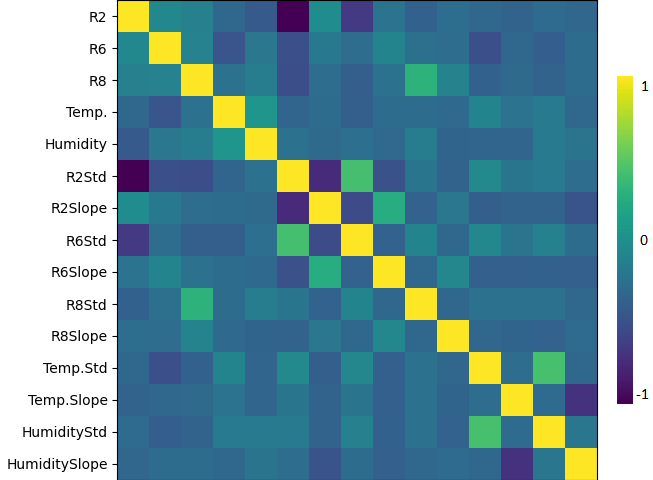
\includegraphics[width=\linewidth]{figuras/Correlation_bien.png}
  \caption{Matriz de correlación después de borrar atributos redundantes.}
  \label{fig:corrBien}
\end{minipage}
\end{figure}
\noindent
Podemos ver que los sensores R1, R2, R3 y R4 están muy fuertemente correlacionados. Lo mismo ocurre entre los sensores R7 y R8. Por ello, hemos elegido quedarnos únicamente con los sensores R2, R6 y R8. Existen otras redundancias entre algunos de los atributos estadísticos introducidos y sus respectivos sensores. En particular podemos fijarnos que cada sensor es redundante con sus atributos de Mean, Min y Max, por lo que se van a eliminar del dataset. Estos arreglos resultan en una matriz de correlación ideal (Figura \ref{fig:corrBien}), en la que las únicas correlaciones altas son entre un atributo y él mismo.
\newline\newline
Haber pasado de 54 atributos a 15 favorece entrenamientos más efectivos y reduce considerablemente los tiempos de ejecución para cualquier clasificador a probar. La eliminación de estos atributos no afecta a la precisión de los clasificadores ya que la información que pueden extraer de ellos es redundante. Los resultados se pueden ver en la Sección \ref{section:results} y su análisis en la Sección \ref{section:resultsAnal}.

\section{Modelos utilizados, descripción del protocolo experimental y estimación de parámetros}
Hemos usado los modelos estudiados en clase de teoría: Naive Bayes \cite{naive_bayes}, K Nearest Neighbors \cite{knn}, Logistic Regression \cite{LogisticRegression}, Red Neuronal \cite{neuralnetwork} y Random Forest \cite{randomforests} de SKLearn \cite{scikit-learn}. Los escogimos tanto por estar familiarizados con ellos, como porque son capaces de tratar con problemas multiclase (excepto la regresión lineal, pero SKLearn. tiene un parámetro que permite usar el algoritmo 'one vs rest' para hacer una clasificación multiclase). De los diferentes tipos de Naive Bayes que existen escogimos el gausiano, ya que todos los atributos de los datos que vamos a tratar son continuos.

\clearpage
\noindent
El protocolo experimental usado ha consistido en probar en cada clasificador sus hiperparámetros más importantes:
\begin{itemize}[noitemsep]
\item Naive Bayes: Ninguno.
\item KNN: Número de vecinos.
\item Logistic Regresion: Ninguno.
\item Red Neuronal: Número de capas ocultas (1-2) y neuronas por capa (10-40). Por simplicidad siempre usamos el mismo número de neuronas en ambas capas.
\item Random Forest: Número de estimadores.
\end{itemize}
\noindent
Para el cálculo de la precisión se utiliza la función cross\_val\_score de SKLearn para hacer una validación cruzada de 5 iteraciones. Esto se realiza para evitar el sobreajuste. Cross\_val\_score se encarga de hacer la separación de los datos de entrenamiento y de prueba en cada iteración automáticamente. Para los clasificadores para los que es necesario (o aconsejable) normalizar los datos, usamos una pipeline de SKLearn que normaliza las particiones de datos de entrenamiento y prueba en cada iteración de la validación cruzada antes de clasificar.
\newline\newline
Por último, para acelerar el tiempo de ejecución del fichero que prueba los parámetros usamos el módulo Multiprocessing de Python  \cite{multiprocessing} para distribuir la carga entre varios núcleos.


\section{Resultados obtenidos}\label{section:results}
\begin{table}[H]
  \centering
        \begin{tabular}{|c|c|}
        \hline
        \multicolumn{2}{|c|}{\text{Gauss. Naive Bayes}} \\
        \hline        
        \hline
          Accur. &     Desv \\
        \hline
        0.565277 & 0.002953 \\
        \hline
        \end{tabular}
        \quad
        \begin{tabular}{|c|c|}
        \hline
        \multicolumn{2}{|c|}{\text{Regresión Logística}} \\
        \hline
        \hline
          Accur. &     Desv \\
        \hline
        0.678291 & 0.001224 \\
        \hline
        \end{tabular}
        \quad
        \begin{tabular}{|c|c|c|}
        \hline
        \multicolumn{3}{|c|}{\text{KNN}} \\
        \hline        
        \hline
         K &   Accur. &     Desv \\
        \hline
         3 & 0.9863 & 0.000628 \\
         8 & 0.9739 & 0.000723 \\
        13 & 0.9601 & 0.000957 \\
        18 & 0.9542 & 0.000892 \\
        38 & 0.9313 & 0.001110 \\
        \hline
        \end{tabular}
        \quad
        \begin{tabular}{|ll|c|c|}
        \hline
        \multicolumn{4}{|c|}{\text{Red Neuronal}} \\
        \hline
        \hline
        Capas & Neuronas & Accur. & Desv \\
        \hline
        1 & 10 &  0.813982 &  0.004911 \\
          & 20 &  0.863128 &  0.009472 \\
          & 30 &  0.892082 &  0.005235 \\
          & 40 &  0.912408 &  0.003810 \\
        \hline
        2 & 10 &  0.864355 &  0.009236 \\
          & 20 &  0.946296 &  0.002155 \\
          & 30 &  0.969213 &  0.003137 \\
          & 40 &  0.979955 &  0.001634 \\
        \hline
        \end{tabular}
        \quad
        \begin{tabular}{|c|c|c|}
        \hline
        \multicolumn{3}{|c|}{\text{Random Forest}} \\
        \hline
        \hline
         N &   Accur. &     Desv \\
        \hline
               10 & 0.995373 & 0.000482 \\
               30 & 0.995975 & 0.000407 \\
               70 & 0.996090 & 0.000383 \\
               90 & 0.996182 & 0.000313 \\
              110 & 0.996233 & 0.000522 \\
              130 & 0.996063 & 0.000412 \\
              170 & 0.996154 & 0.000454 \\
        \hline
        \end{tabular}
    \caption{Precisiones y desviaciones típicas de los experimentos de ajuste de hiperparámetros.}
    \label{table:precisionesystd}
\end{table}

\begin{figure}[H]
\centering
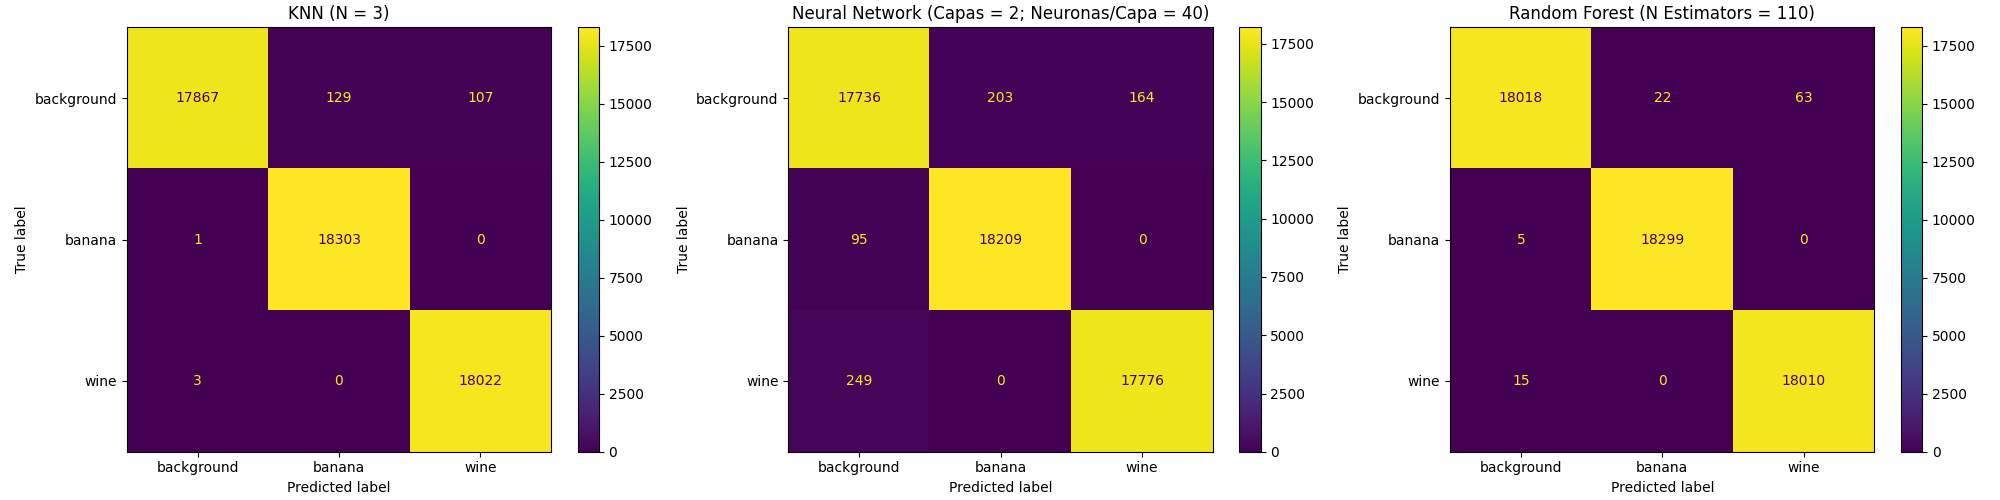
\includegraphics[width=\linewidth]{figuras/confusion_matrix.png}
\caption{Matrices de confusión de los 3 mejores clasificadores.}\label{fig:confusionmatrix}
\end{figure}

\begin{table}[H]
\centering

    \begin{tabular}{|c|c|}
    \hline
    \multicolumn{2}{|c|}{\text{KNN}} \\
    \hline
    \hline
    K &   Accur.\\
    \hline
    3 & 0.948 \\
    8 & 0.921 \\
    13 & 0.901 \\
    28 & 0.869 \\
    \hline
    \end{tabular}
    \quad
    \begin{tabular}{|ll|c|c|}
    \hline
    \multicolumn{3}{|c|}{\text{Red Neuronal}} \\
    \hline
    \hline
    Capas & Neuronas & Accur.\\
    \hline
    1& 20 &  0.846 \\
    & 40 &  0.887 \\
    2& 20 &  0.915 \\
    & 40 &  0.952 \\
    \hline
    \end{tabular}
    \quad
    \begin{tabular}{|c|c|c|}
    \hline
    \multicolumn{2}{|c|}{\text{Random Forest}} \\
    \hline
    \hline
    N &   Accur.\\
    \hline
        10 & 0.971\\
        30 & 0.973\\
        110 & 0.974\\
        170 & 0.974\\
    \hline
    \end{tabular}
    \caption{Precisiones de los mejores clasificadores usando 1/10 de los datos.}
    \label{table:menosdatos}
\end{table}
En las Tablas \ref{table:precisionesystd} y \ref{table:menosdatos}, y en la Figura \ref{fig:confusionmatrix}, tenemos los resultados de los experimentos realizados.


\section{Discusión de los resultados obtenidos y conclusiones}\label{section:resultsAnal}
Como se puede ver en la tabla \ref{table:precisionesystd}, los 3 clasificadores que mejor precisión consiguieron (independientemente de sus hiperparámetros), fueron los clasificadores KNN, Neural Network y Random Forest. Las tablas expuestas son los algoritmos más representativos de los que probamos, hicimos más pruebas pero no son relevantes y ocuparían espacio de más.
\newline\newline
Viendo todos los clasificadores y como varía la precisión según su funcionamiento o la variación de los hiperparámetros deja entrever que nuestro dataset requiere de un modelo muy complejo con muchos parámetros y una frontera de decisión que dista mucho de ser simple o necesitar regularización.
\newline\newline
La variación de la precisión cuando vamos aumentando la cantidad de vecinos en KNN confirma nuestra hipótesis, cuantos más vecinos, la frontera de decisión se simplifica (hace como un efecto de regularización). Eso quiere decir que 3 vecinos es el más apropiado porque permite un modelo mucho más complejo.
\newline\newline
Logistic Regression requiere que los datos sean linealmente separables, esa es la razón por la que se comporta tan erráticamente. Naive Bayes, aun que no separa los datos linealmente también genera un modelo demasiado simple.
\newline
El mejor resultado en las redes neuronales se obtiene con la configuración más compleja probada, con 2 capas y 40 neuronas por capa.
\newline\newline
El caso de Random Forest es diferente. Aunque el que mejor rendimiento da es el que tiene 110 estimadores, la diferencia al variar el hiperparámetro es despreciable y podría ser debida a la aleatoriedad del algoritmo. Un árbol de decisión ya de por si puede generar una frontera de decisión muy compleja, pero si esto lo combinamos con que en Random Forest los árboles votan usando bagging y se contrarrestan los errores entre ellos tenemos que es el que mejor resultado da repetidamente. Si nos fijamos en la Figura \ref{fig:confusionmatrix} vemos cómo, además de ser el que mejor precisión obtiene, es muy bueno distinguiendo entre vino y plátano y se comporta mejor que la red neuronal.
\newline\newline
Como ya hemos dicho, este dataset requiere de modelos muy complejos, pero aún así nos parece que obtenemos un rendimiento más que aceptable y es difícil imaginar una situación en la que Random Forest no sea el mejor, ya que es rápido, prácticamente no requiere de ajuste de hiperparámetros y obtiene resultados muy fiables.
\newline\newline
KNN también es un buen clasificador con 3 vecinos. En cambio, su complejidad computacional es mucho mayor a Random Forest. Si quisiéramos construir un sistema que detecte en tiempo real qué alimento se encuentra en la sala, el uso de KNN no es adecuado por su elevado tiempo de ejecución. En su favor hay que decir que viendo la matriz de confusión (Figura \ref{fig:confusionmatrix}), es el algoritmo que menos confunde los objetos a detectar (vino y plátano). KNN tiene un mayor error clasificando erróneamente el ruido de fondo, pero si le quisiéramos dar prioridad a detectar cualquier tipo de alimento frente a diferenciarlos entre sí, podría interesarnos más KNN. Aún así opinamos que un Random Forest es más adecuado para el problema que queremos solucionar.
\newline\newline
El dataset que usamos tiene una cantidad muy elevada de datos, por lo que hemos comprobado cómo se comportarían los modelos elegidos con muchos menos datos. Ejecutando los mismos experimentos para 1/10 de los datos (salvo algunos hiperparámetros que inferimos que no van a rendir muy bien vistos los resultados anteriores), obtenemos las precisiones de la Tabla \ref{table:menosdatos}. Como se puede observar, Random Forest sigue dominando sobre el resto. De hecho, es el algoritmo que menos perjudicado se ve por la drástica reducción del volumen de los datos. En cuanto a las matrices de confusión, observamos que se mantiene la misma tendencia salvo que ahora Random Forest es también el mejor diferenciando entre Vino y Plátano, nulificando la única ventaja que KNN tenía sobre este.
\newline\newline
En conclusión, vistos los resultados de la Sección \ref{section:results} y el análisis de los mismos realizado en esta, el algoritmo que utilizaríamos para clasificar instantes de tiempo es Random Forest, con un número de estimadores igual a 110.

% ****************************************************************************
% BIBLIOGRAPHY AREA
% ****************************************************************************

\begin{footnotesize}

% IF YOU DO NOT USE BIBTEX, USE THE FOLLOWING SAMPLE SCHEME FOR THE REFERENCES
% ----------------------------------------------------------------------------
%\begin{thebibliography}{99}
%
% For books
%\bibitem{Haykin_book} S. Haykin, editor. \emph{Unsupervised Adaptive Filtering vol.1 : Blind Source Separation}, John Willey ans Sons, New York, 2000.
%
% For articles
%\bibitem{DelfosseLoubaton_article}N. Delfosse and P. Loubaton, Adaptibe blind separation of sources: A deflation
%approach, \emph{Signal Processing}, 45:59-83, Elsevier, 1995.
%
%% For paper in proceedings published as serie books (LNCS,...)
%\bibitem{CrucCichAmari_bookproceedings} S. Cruces, A. Cichocki and S. Amari, The minimum entropy and cumulants based contrast functions for blind source extraction. In J. Mira and A. Prieto, editors, proceedings of the 6$^{th}$ \emph{international workshop on artificial neural networks} ({IWANN} 2001), Lecture Notes in Computer Science 2085, pages 786-793,
%Springer-Verlag, 2001.
%
%% For paper in conference proceedings
%\bibitem{VrinsArchambeau_proceedings} F. Vrins, C. Archambeau and M. Verleysen, Towards a local separation performances estimator using common ICA contrast functions? In M. Verleysen, editor, \emph{proceedings of the $12^{th}$
%European Symposium on Artificial Neural Networks} ({ESANN} 2004),
%d-side pub., pages 211-216, April 28-30, Bruges (Belgium), 2004.
%
%% For Technical Report
%\bibitem{Stone_TechRep} J. V. Stone and J. Porrill, Undercomplete independent component analysis for signal separation and dimension
%reduction. Technical Report, Psychology Department, Sheffield
%University, Sheffield, S10 2UR, England, October 1997.
%\end{thebibliography}
% ----------------------------------------------------------------------------

% IF YOU USE BIBTEX,
% - DELETE THE TEXT BETWEEN THE TWO ABOVE DASHED LINES
% - UNCOMMENT THE NEXT TWO LINES AND REPLACE 'Name_Of_Your_BibFile'
\clearpage
\bibliographystyle{unsrt}
\bibliography{mi_bibliografia}

\end{footnotesize}

% ****************************************************************************
% END OF BIBLIOGRAPHY AREA
% ****************************************************************************

\end{document}
